\documentclass[11pt]{article}
\usepackage[left=1.75cm,right=1.75cm,top=1.5cm,bottom=2cm]{geometry}
\usepackage{fontspec}
\usepackage{graphicx}
\usepackage{eso-pic}
\usepackage{amsmath}  % improve math presentation
\usepackage{amsfonts}
\usepackage{amsthm}
\usepackage{tabularx}
\usepackage{longtable}
\usepackage{array}
\usepackage{booktabs}
\usepackage{caption}


\usepackage{hyperref} % Add this line for the \url command
\hypersetup{
	colorlinks=true,       % false: boxed links; true: colored links
	linkcolor=black,        % color of internal links,
	citecolor=black,
}

\setmainfont{Calibri}
\linespread{1.15}

% ++++++++++++++++++++++++++Code global config begin++++++++++++++++++++++++++
% Code block universal settings, all lstdefinestyle must appeared below this block!
\usepackage{listings}
% use txtt global font
% \usepackage[T1]{fontenc} % Add font options

\DeclareFixedFont{\codefont}{T1}{txtt}{m}{n}{12} % other options: txtt -> cmtt, pcr, fvm, zi4; m -> bx, n; 12 -> (fontsize)

% Define colors
\usepackage{color}
\usepackage{tikz} % colorlet need this
\definecolor{commentgreen}{rgb}{0,0.5,0}
\colorlet{framegray}{black!40}
\definecolor{stringred}{rgb}{0.6,0,0}

% Global config
\lstset{
	backgroundcolor=\color{gray!7},
	numbers = left, % show line number on the left
	numberstyle = \small\color{framegray}, % line number color
	basicstyle = \codefont, % code font
	columns = flexible, % make the spacing between characters compact
	keepspaces = true,  % keeps spaces in text, useful for keeping indentation of code (needs columns=flexible)
	% captionpos = b, % caption at the bottom
	commentstyle = \color{commentgreen}, % comment color
	frame = single, % display frame
	stringstyle = \color{stringred}, % Strings in red
	rulecolor = \color{framegray}, % frame color
	showstringspaces = false, % don't mark spaces in strings
	breaklines = true, % break long lines
	tabsize = 4, % tab size
}
% +++++++++++++++++++++++++++Code global config end+++++++++++++++++++++++++++

% ++++++++++++++++++++++++++VHDL local config begin++++++++++++++++++++++++++
% Must placed below the global settings
% Custom colors for VHDL only
\usepackage{textcomp}
\definecolor{emph1purple}{RGB}{128, 0, 128}
\definecolor{emph2red}{RGB}{200, 20, 0}
\colorlet{keywordblue}{blue!100!black!80}
% this will override the global settings
\lstdefinestyle{customvhdl}{
	language = VHDL,
	emph = {std_logic, STD_LOGIC, std_logic_vector, STD_LOGIC_VECTOR, std_logic_1164, STD_LOGIC_1164}, % Custom highlighting
	emphstyle = \color{emph1purple},  % Highlighted words in pink
	emph={[2]XNOR, xnor, xor, XOR, nand, NAND, nor, NOR, not, NOT, and, AND, or, OR}, % Custom highlighting
	emphstyle = {[2]\color{emph2red}},  % Highlighted words in green
	keywordstyle = \color{keywordblue},
	morecomment=[l]{--},
	morekeywords={
		library, LIBRARY, use, USE, all, ALL, entity, ENTITY, is, IS, port, PORT, map, MAP, in, IN, out, OUT, end, END, architecture, ARCHITECTURE, of, OF, begin, BEGIN, signal, SIGNAL
	}
}
% ++++++++++++++++++++++++++++VHDL local config end++++++++++++++++++++++++++++



\AddToShipoutPictureBG*{%
    \AtPageLowerLeft{%
        \raisebox{0.5cm}{\makebox[2cm\ \ \ \ \ \ \ \ \ \ \ \ \ \ \ \ \ \ \ ][l]{\includegraphics[width=4cm]{logo.jpg}}}
    }
}

% Ensure 11pt font size
\AtBeginDocument{\fontsize{11pt}{13pt}\selectfont}
\begin{document}

\noindent \textbf{Course: }UESTC3020 \\
\noindent \textbf{Names: }Jinming Ren, Yuhao Liu (Both from class 4) \\
\noindent \textbf{GUIDs: }2840216R, 2840218L \\
\noindent \textbf{Date:} 12 January 2024 \\

\noindent \Large{\textbf{DCD Coursework Report}}
\vspace{-0.5em}

\fontsize{11pt}{11pt}\selectfont
\linespread{1}

\section{PART II: Validation of Combinational Design}

The circuit structure of the 2-bit and 4-bit adder are shown in Figure~\ref{fig:2bit_adder} and Figure~\ref{fig:4bit_adder} in Appendix~\ref{app:a} respectively.

\subsection{Task 7-8: VHDL Behavioural Description and Simulation of the 2-bit Adder}
\label{sec:task78}

Listing~\ref{lst:2bit_adder} in Appendix~\ref{app:c} contains the behavioural description of the 2-bit adder. We simulate\footnote{All testbench files can be seen at \url{https://github.com/Marcobisky/dcd-generalized-adder}} the 2-bit adder with 4 test cases: $00+00$, $01+01$, $10+10$, and $11+11$. The output waveform is shown in Figure~\ref{fig:2bit_adder_waveform}.

\subsection{Task 9-10: VHDL Structural Description and Simulation of the 4-bit Adder}

We reuse the design of the 2-bit adder in Section~\ref{sec:task78} to build the 4-bit adder. The structural description of it is shown in Listing~\ref{lst:4bit_adder} in Appendix~\ref{app:c}. We simulate the 4-bit adder with 5 test cases: $0000+0000$, $0001+0001$, $1111+0001$, $1010+0101$, and $1111+1111$. The output waveform is shown in Figure~\ref{fig:4bit_adder_waveform}, which shows that the result is $0000$ (\texttt{c=0}), $0010$ (\texttt{c=0}), $0000$ (\texttt{c=1}), $1111$ (\texttt{c=0}), and $1110$ (\texttt{c=1}) respectively. Obviously, they are correct.

\section{PART III: Generalised Adder}

\subsection{Task 11: Block Diagram of Our Proposed Generalised Adder}
\label{sec:task11}

The block diagram of our proposed generalised adder is shown in Figure~\ref{fig:block_diagram} in Appendix~\ref{app:b}. Here is an explanation of each block in the diagram and how they are connected each other:

\begin{itemize}
	\item \textbf{Input:} For the user to enter the number of data $N$ and all operands.
	\item \textbf{Data Storage Part:} Store N 4-bit data entered by the user and transmit them to the adder one by one with 4 bits transmitted in parallel.
	\item \textbf{4-bit Adder/Counter:} Considering the various possible forms of the final output and the rules for adding $N$ 4-bit data, we decompose the addition between them into that for the first four bits and the last four bits. For the addition of the first four bits, we use the memory part to store the result of the previous operation and add it to the new input, and each resulting carry is entered into the adder for the last four bits for accumulation.
	\item \textbf{Connector:} Reassemble the 8 bits of the operation result.
	\item \textbf{FSM (Control Unit):} Provide all control signals and the clock signal. (Ensure that the circuit can run when $N$ data have been inputted and stored and the final outcome can be presented when and only when N data have participated in operation.)
	\item \textbf{Output:} Display the final result.
\end{itemize}

\subsection{Task 12: Realization of Each Block in Section~\ref{sec:task11}}

The circuit realization of the proposed generalised adder is shown in Figure~\ref{fig:main} in Appendix~\ref{app:b}.

\subsection{Task 13-14: VHDL Behavioural Description and Simulation of Each Block in Section~\ref{sec:task11}}

All the behavioural descriptions of the proposed generalised adder is shown in Appendix~\ref{app:c2}. All  The simulation\footnote{All testbench files in VHDL can be seen at \url{https://github.com/Marcobisky/dcd-generalized-adder}} methods and results are presented in sections below\footnote{Only part of the FSM (Control Unit) block (\texttt{isMax}) is simulated here, other parts are simulated in Section~\ref{sec:task1516}.}.

\subsubsection{Counter (Higher 4 bits adder)}

According to the specifications in Section~\ref{sec:task11}, this counter should be able to add one whenever the result of the lower 4 bits have a carry. The simulation waveform in Figure~\ref{fig:RhCount_waveform} in Appendix~\ref{app:b-2} is explained as follows:

\begin{enumerate}
	\item 0 ns: The counter is initialized to 0.
	\item 0-30 ns: The counter keeps its value because the \texttt{c} signal is not asserted.
	\item 30-80 ns: \texttt{c} signal is asserted at 30 ns, the counter increases by one at 40 ns and 60 ns where the clock is a rising edge.
	\item 80-110 ns: Same as step 2.
	\item 110-140 ns: Same as step 3.
\end{enumerate}

\subsubsection{Connector}

According to the specifications in Section~\ref{sec:task11}, this connector should be able to reassemble the lower and higher 4 bits of the operation result. The simulation waveform in Figure~\ref{fig:buffer8bit_waveform} in Appendix~\ref{app:b-2} is explained as follows:

\begin{enumerate}
	\item 0 ns: \texttt{rh} and \texttt{rl} is initialized to 0x0A and 0x05 respectively.
	\item 0-30 ns: The connector keeps its value because the \texttt{rst} signal\footnote{Though this \texttt{rst} signal is called ``reset'', in the case of this \texttt{connector}, it makes the final calculation visible at the end of calculation. For other modules, this \texttt{rst} clear the memory inside.} is not asserted.
	\item 30-60 ns: \texttt{rst} signal is asserted at 30 ns, so the connector immediately shows the assembled result 0xA5.
	\item 60-120 ns: The connector losts its value at 60 ns because the \texttt{rst} signal is unasserted.
\end{enumerate}

\subsubsection{Data Storage Part (EEPROM)}

According to the specifications in Section~\ref{sec:task11}, the user first store all the operand data here before running the calculations. The simulation waveform in Figure~\ref{fig:EEPROM_waveform} in Appendix~\ref{app:b-2} is explained as follows:

\begin{enumerate}
	\item 0-10 ns: The stored data in address 0x00 contains a random value (which happens to be 0x00). Write enable (\texttt{we}) signal is unasserted.
	\item 10-40 ns: \texttt{we} signal is asserted at 10 ns, the data 0x0A is written into address 0x00.
	\item 40-120 ns: \texttt{we} signal is unasserted at 40 ns, therefore, as long as the address line is not changed, the data in address 0x00 is always 0x0A.
	\item 120-130 ns: The address line is changed to 0x01, the output \texttt{dout} is showing the number randomly initialized in that address.
	\item 130-150 ns: \texttt{we} signal is asserted at 130 ns. The data 0x0C is written into address 0x01 at 130 ns because the clock is rising edge.
	\item 150-190 ns: Same as step 3.
\end{enumerate}

\subsubsection{\texttt{isMax} module (Part of the FSM)}

This module should be able to determine whether the calculation is finished (i.e., if the \texttt{addr} signal is exactly equal to the predefined \texttt{n} value). The simulation waveform in Figure~\ref{fig:isMax_waveform} in Appendix~\ref{app:b-2} is explained as follows:

\begin{enumerate}
	\item 0-10, 30-40 ns: \texttt{addr} is exactly equal to \texttt{n}. Therefore, the \texttt{rst} signal is asserted.
	\item 10-30, 40-50 ns: \texttt{addr} is not equal to \texttt{n}. Therefore, the \texttt{rst} signal is unasserted.
\end{enumerate}

\subsection{Task 15-16: VHDL Structural Description and Simulation of Our Complete Generalised Adder}
\label{sec:task1516}

The structural description of the complete system is shown in Listing~\ref{lst:main} in Appendix~\ref{app:c3}. According to the requirements of the task, we simulate the generalised adder with the following case\footnote{The last two numbers in decimal are $7$ and $9$, which are the sum of last two digits of our GUIDs.}:

\begin{itemize}
	\item $N=4+1=5$.
	\item Input 0-3: $0011$, $0101$, $0111$, $1001$. (In decimal, they are $3$, $5$, $7$, $9$)
\end{itemize}

\subsection{Task 17: Simulation Results of Our Generalised Adder}
\label{sec:task17}

The output waveform is shown in Figure~\ref{fig:main_waveform} in Appendix~\ref{app:b-2}. Here is the explanation of the waveform (which works perfectly as expected\footnote{For dynamic and visualized simulation, check out \url{https://github.com/Marcobisky/dcd-generalized-adder} for the \texttt{Digital} source files.}):

\begin{enumerate}
	\item 0 ns: Begin simulation by prompt the user to enter the number of data $N$ (in this case, there are $4$ data, so $N = 4+1 = 5$).
	\item 0-25 ns: Assert \texttt{write} and \texttt{forcerst} signal and wait for a clock period to clear the random memory in \texttt{EEPROM}.
	\item 25-65 ns: Unassert \texttt{write} but keep \texttt{forcerst} asserted to clear the random bits inside all counters and buffers.
	\item 65-145 ns: Assert \texttt{write} signal and unassert \texttt{forcerst} to write the four data together with their corresponding addresses into the \texttt{EEPROM}. (For example, in 65-85 ns, the first data $0011$ (3 in decimal) is written into the address 0.)
	\item 145-230 ns: Unassert \texttt{write} signal and wait for calculation (the \texttt{FSM} will fetch all the data from the \texttt{EEPROM} and calculate their sum, since there are $4$ operands, $4$ clock cycles should be waited).
	\item 230-250 ns: The final result $24$ in decimal (which is the correct sum of $3+5+7+9$) is displayed on the output.
	\item >250 ns: If the user do not assert \texttt{forcerst} signal, the circuit will go back to step 4 and form a loop.
\end{enumerate}

\section{Conclusion}

As can be seen from the circuit structure and simulation results, the universal adder we designed run smoothly and meet all the design requirements, including data input one by one, four bits of each data input in parallel, users can design the number of data involved in the calculation, the final result is output after all the data is involved in the calculation and so on.

For future work, we can further optimize and simplify the construction and connection of various components in the circuit to reduce the integrated complexity. In addition, if the cost of various logic gates and various integrated components is known, we can further reduce the design cost of the entire circuit through calculation. Finally, for better utilization in ANN, we can reuse the circuit and consider designing a more advanced adder that can perform more complex operations.


\newpage
\begin{appendix}

\section{Figures for PART II}
\label{app:a}

\begin{figure}[h!]
	\centering
	\begin{minipage}{0.48\textwidth}
		\centering
		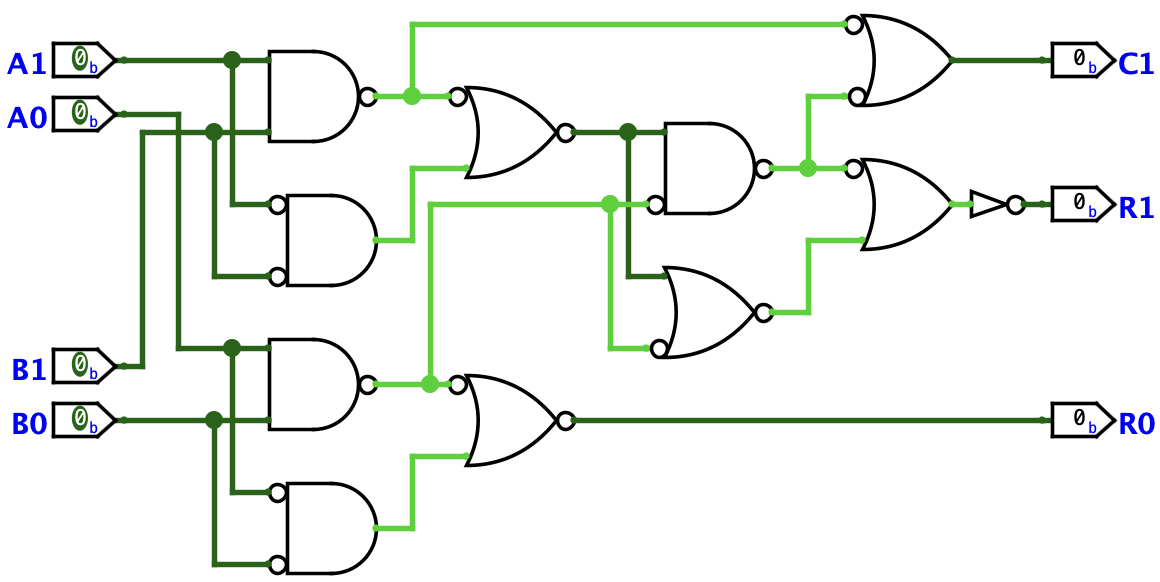
\includegraphics[width=\textwidth]{part1third.png}
		\caption{Circuit Structure of the 2-bit Adder}
		\label{fig:2bit_adder}
	\end{minipage}
	\hfill
	\begin{minipage}{0.48\textwidth}
		\centering
		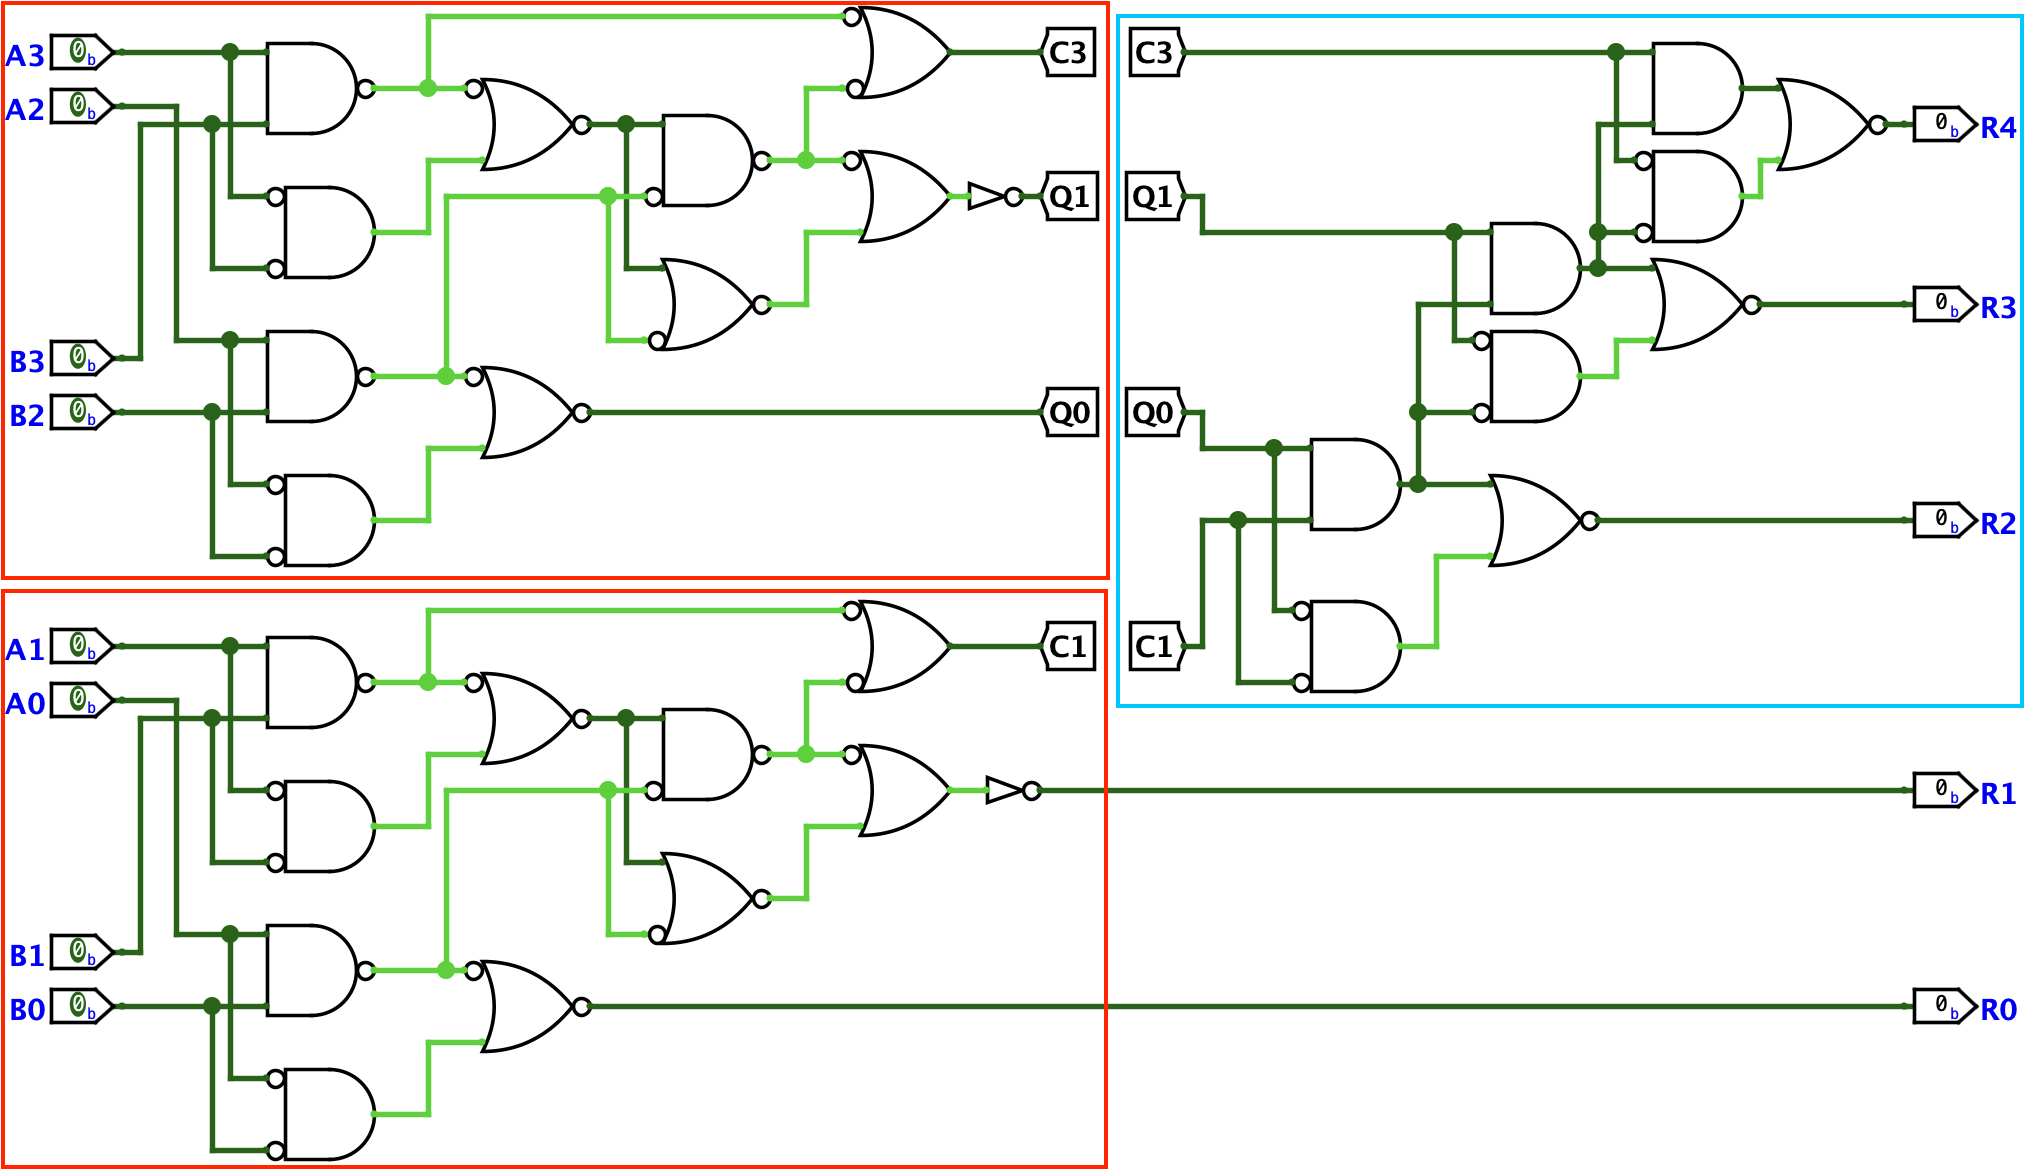
\includegraphics[width=\textwidth]{Part2.png}
		\caption{Circuit Structure of the 4-bit Adder}
		\label{fig:4bit_adder}
	\end{minipage}
\end{figure}

\begin{figure}[h!]
	\centering
	\begin{minipage}{0.45\textwidth}
		\centering
		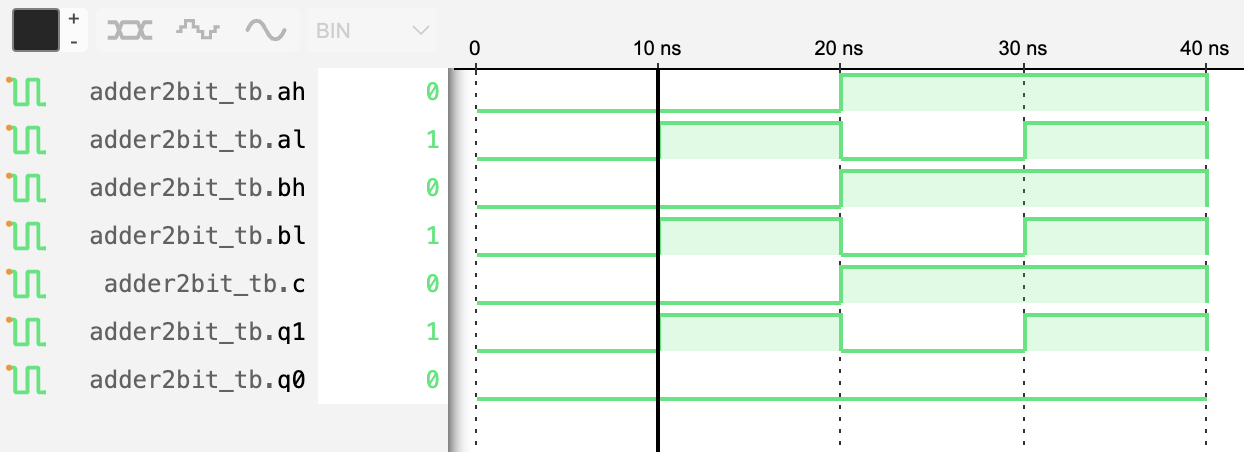
\includegraphics[width=\textwidth]{adder2bit_tb.png}
		\caption{2-bit adder simulation waveform}
		\label{fig:2bit_adder_waveform}
	\end{minipage}
	\hfill
	\begin{minipage}{0.5\textwidth}
		\centering
		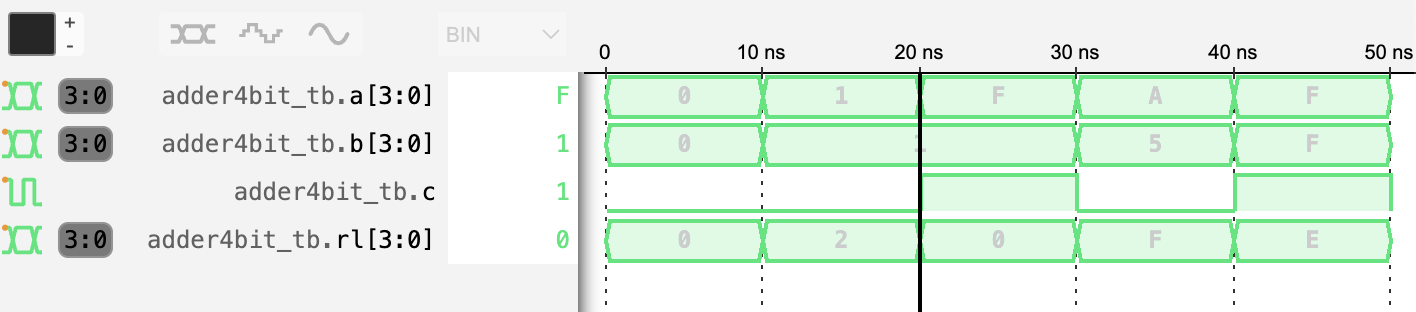
\includegraphics[width=\textwidth]{adder4bit_tb.png}
		\caption{4-bit adder simulation waveform}
		\label{fig:4bit_adder_waveform}
	\end{minipage}
\end{figure}

\section{Circuit Figures for PART III}
\label{app:b}

\begin{figure}[h!]
	\centering
	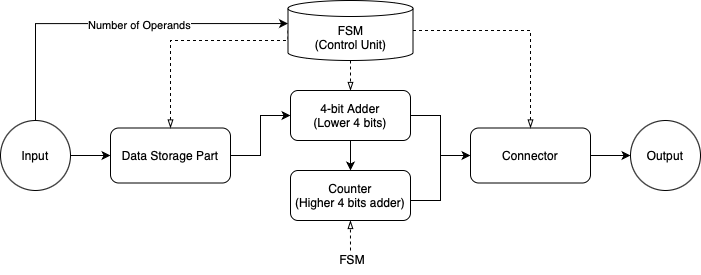
\includegraphics[width=\textwidth]{block-diagram.png}
	\caption[block]{Block diagram of the proposed generalised adder\footnotemark}
	\label{fig:block_diagram}
\end{figure}
\footnotetext{Filled-in arrow denotes data flow, not-filled-in arrow denotes control signals and clock signal.}

\clearpage
\begin{figure}[h!]
	\centering
	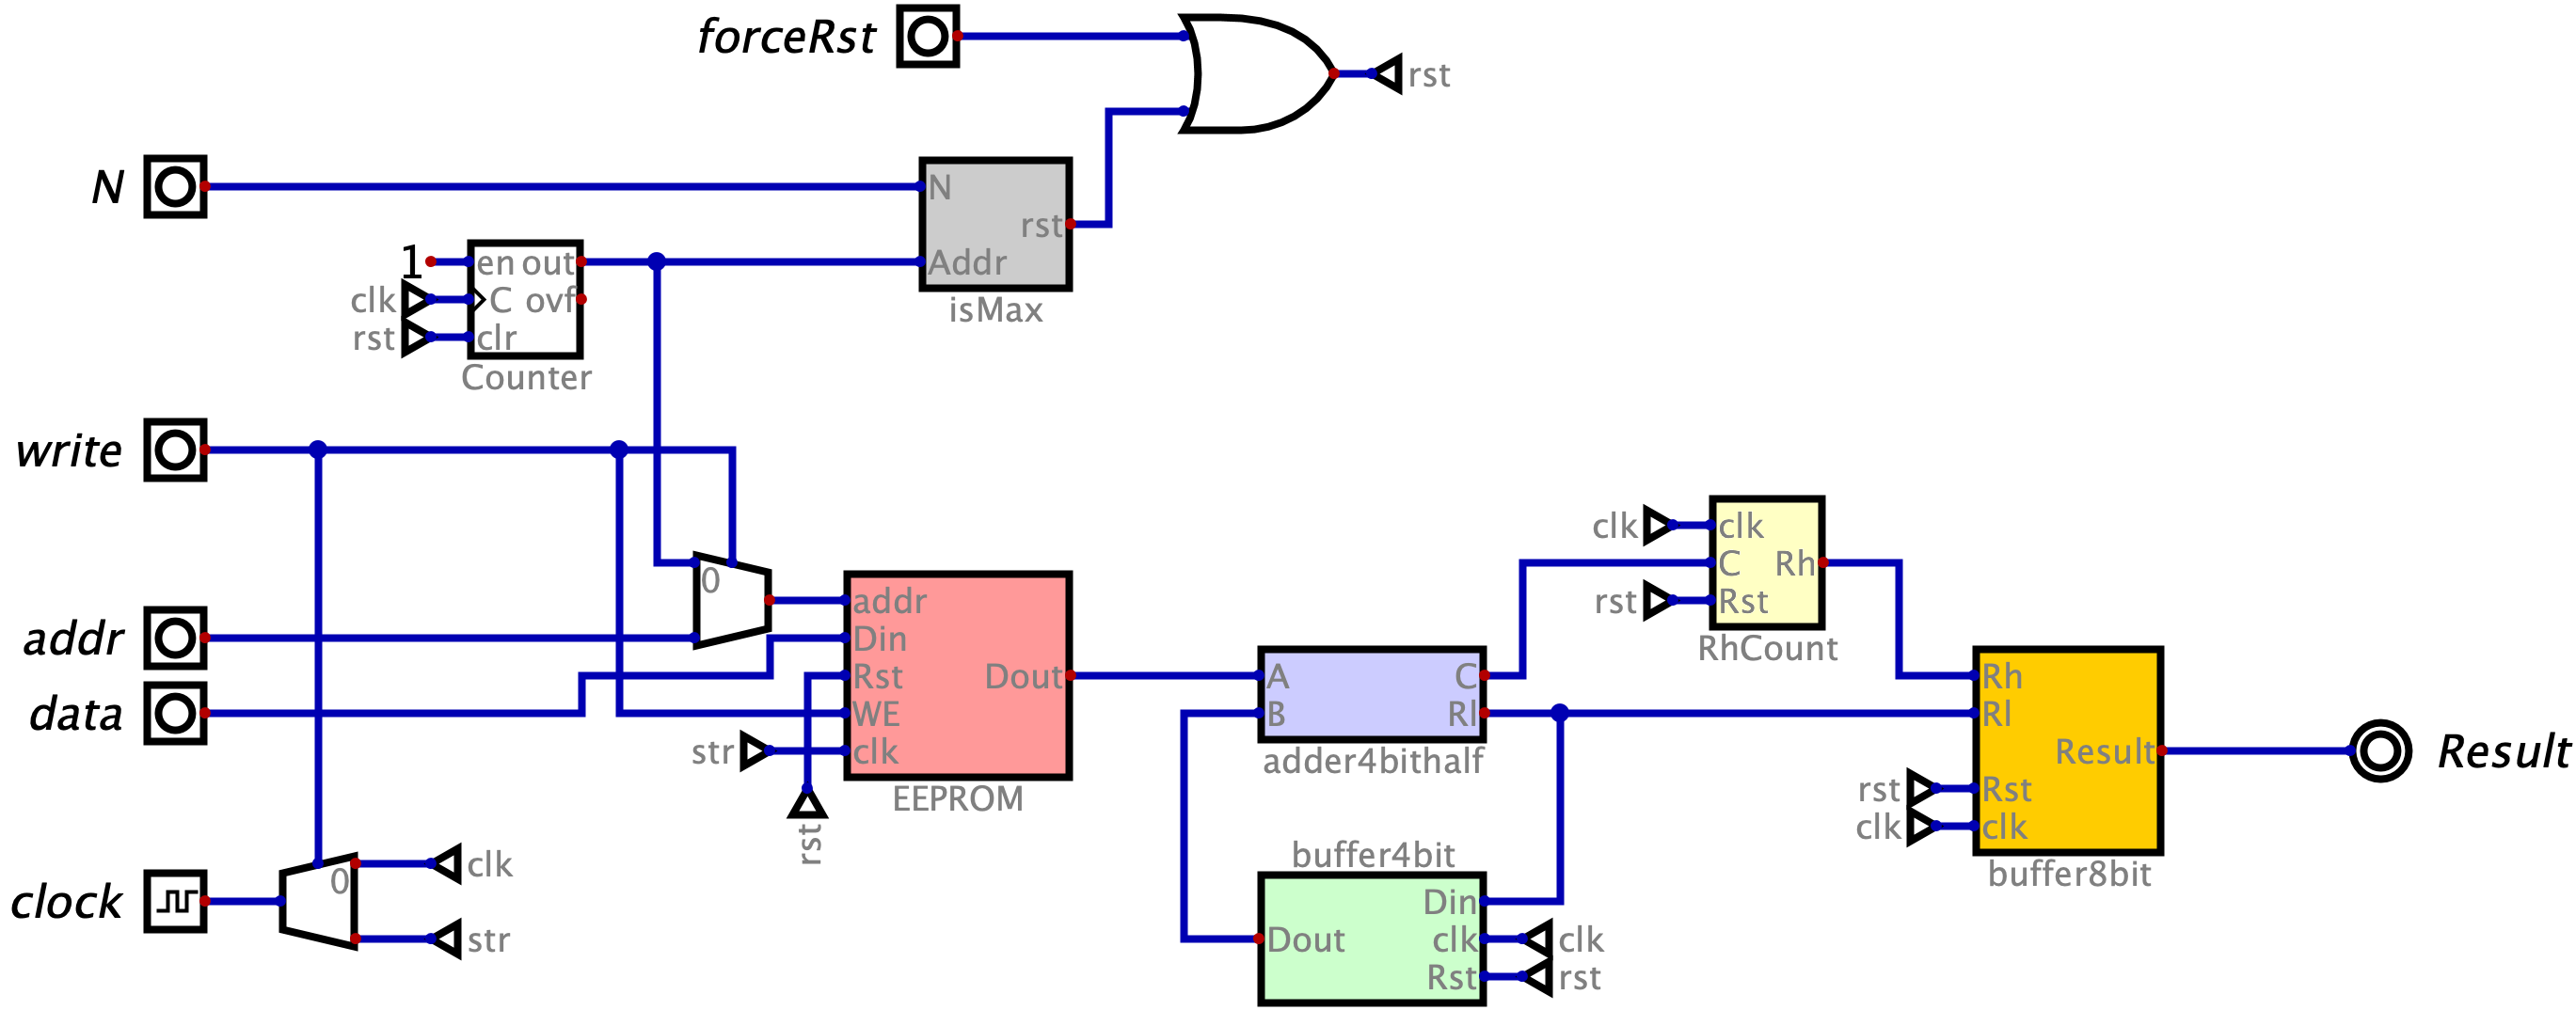
\includegraphics[width=\textwidth]{main.png}
	\caption{Circuit realization of the proposed generalised adder}
	\label{fig:main}
\end{figure}


\section{Simulation Waveforms for PART III}
\label{app:b-2}

\begin{figure}[h!]
	\centering
	\begin{minipage}{0.45\textwidth}
		\centering
		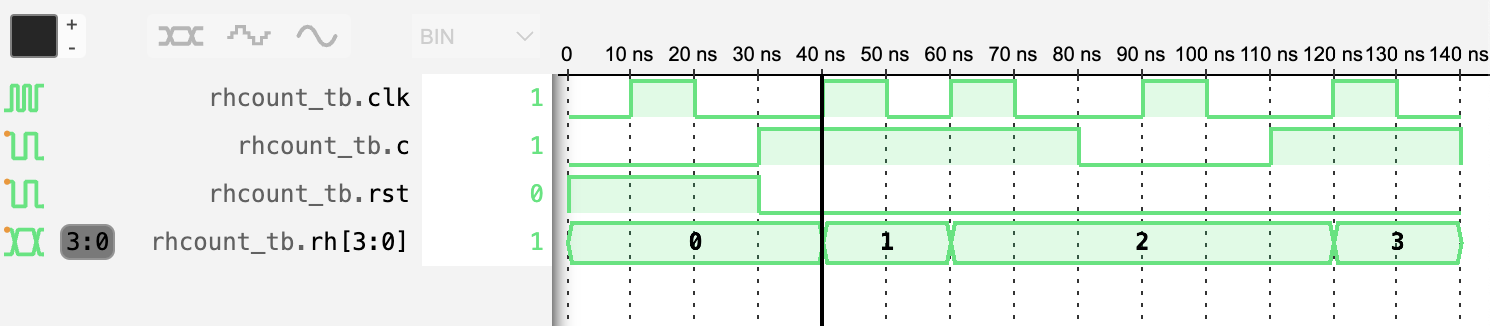
\includegraphics[width=\textwidth]{RhCount_tb.png}
		\caption{Counter (Higher 4 bits adder) simulation waveform}
		\label{fig:RhCount_waveform}
	\end{minipage}
	\hfill
	\begin{minipage}{0.45\textwidth}
		\centering
		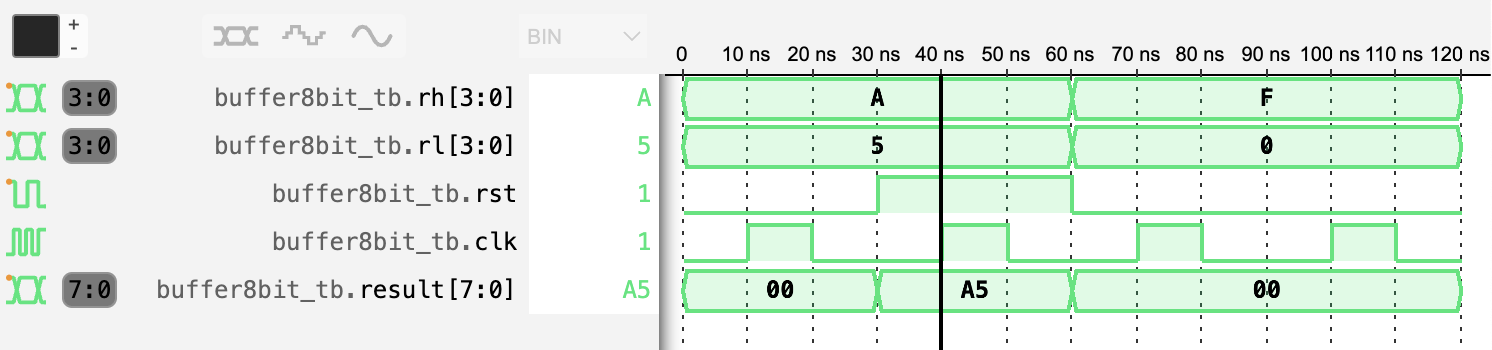
\includegraphics[width=\textwidth]{buffer8bit_tb.png}
		\caption{Connector simulation waveform}
		\label{fig:buffer8bit_waveform}
	\end{minipage}
\end{figure}

\begin{figure}[h!]
	\centering
	\begin{minipage}{0.45\textwidth}
		\centering
		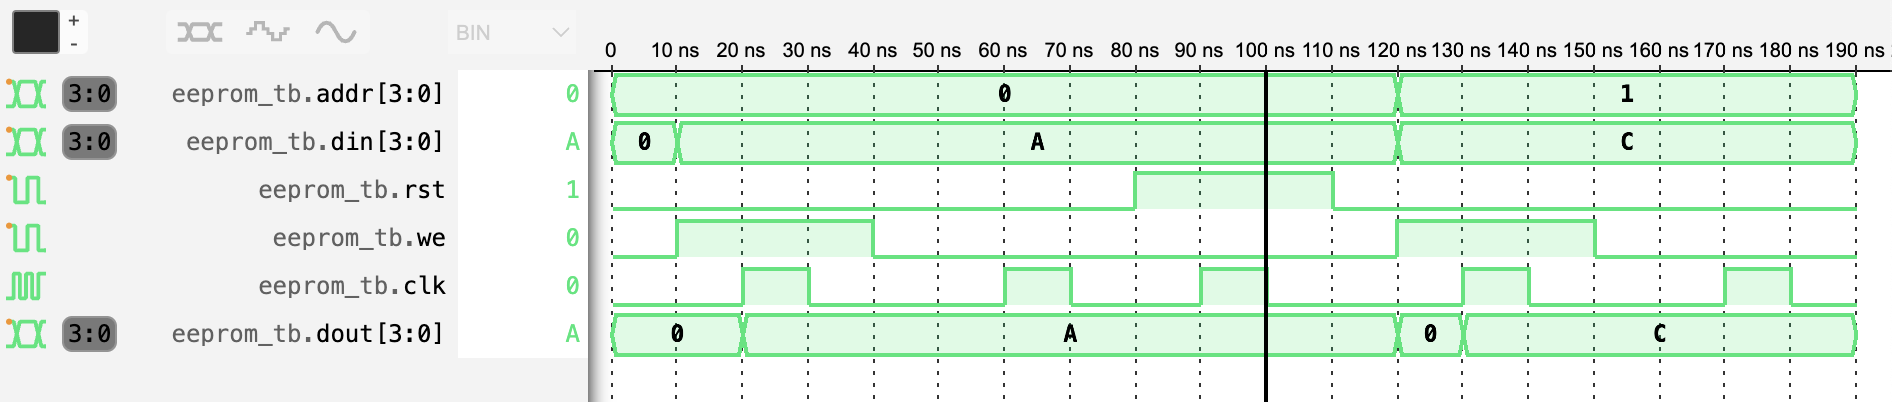
\includegraphics[width=\textwidth]{EEPROM_tb.png}
		\caption{Data Storage Part (EEPROM) simulation waveform}
		\label{fig:EEPROM_waveform}
	\end{minipage}
	\hfill
	\begin{minipage}{0.45\textwidth}
		\centering
		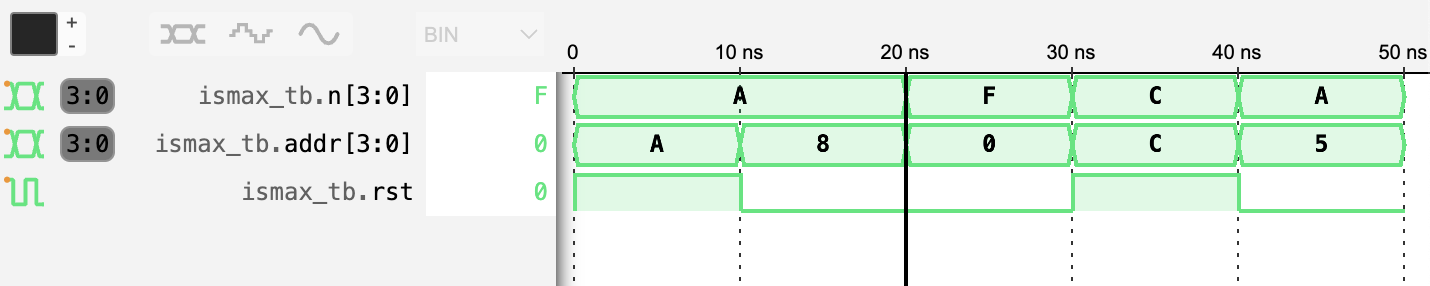
\includegraphics[width=\textwidth]{isMax_tb.png}
		\caption{\texttt{isMax} module (Part of the FSM) simulation waveform}
		\label{fig:isMax_waveform}
	\end{minipage}
\end{figure}

\begin{figure}[h!]
	\centering
	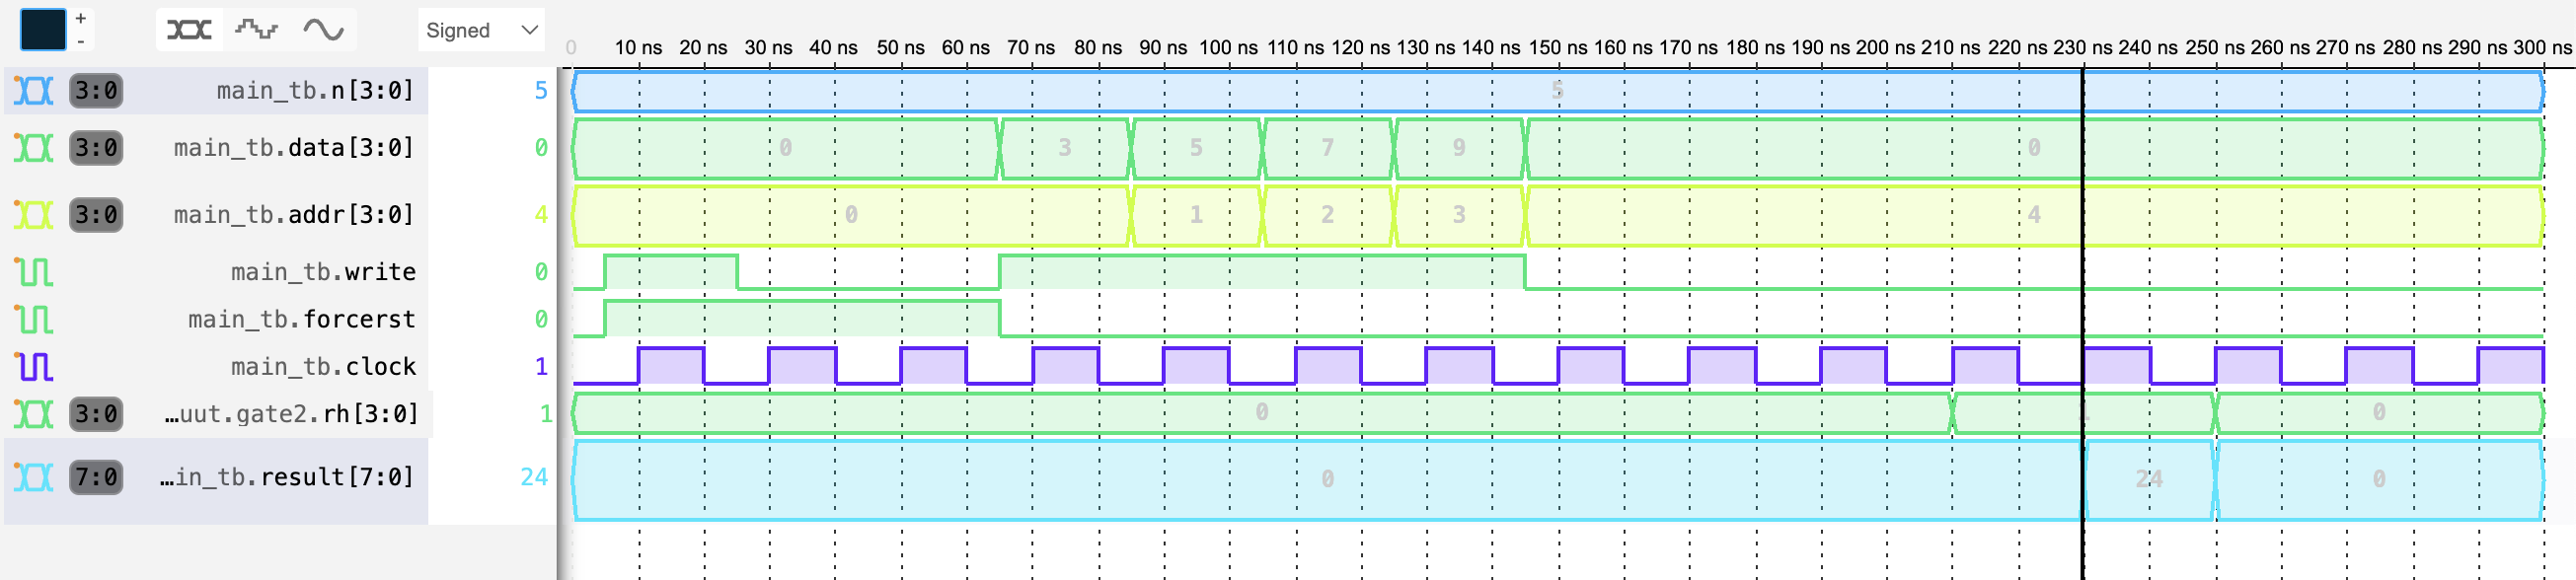
\includegraphics[width=\textwidth]{main_tb.png}
	\caption{Simulation waveform of the proposed generalised adder under the condition specified in Section~\ref{sec:task1516}}
	\label{fig:main_waveform}
\end{figure}

\clearpage
\section{Subcircuit Figures for PART III}
\label{app:subcircuitfigures}

\begin{figure}[h!]
	\centering
	\begin{minipage}{0.45\textwidth}
		\centering
		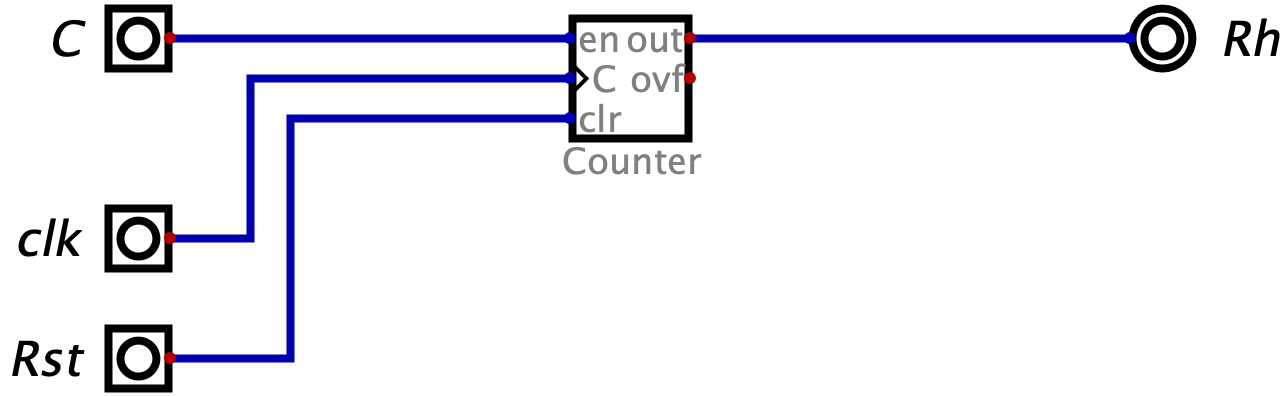
\includegraphics[width=\textwidth]{RhCount.png}
		\caption{Counter (Higher 4 bits adder) subcircuit}
		\label{fig:RhCount}
	\end{minipage}
	\hfill
	\begin{minipage}{0.45\textwidth}
		\centering
		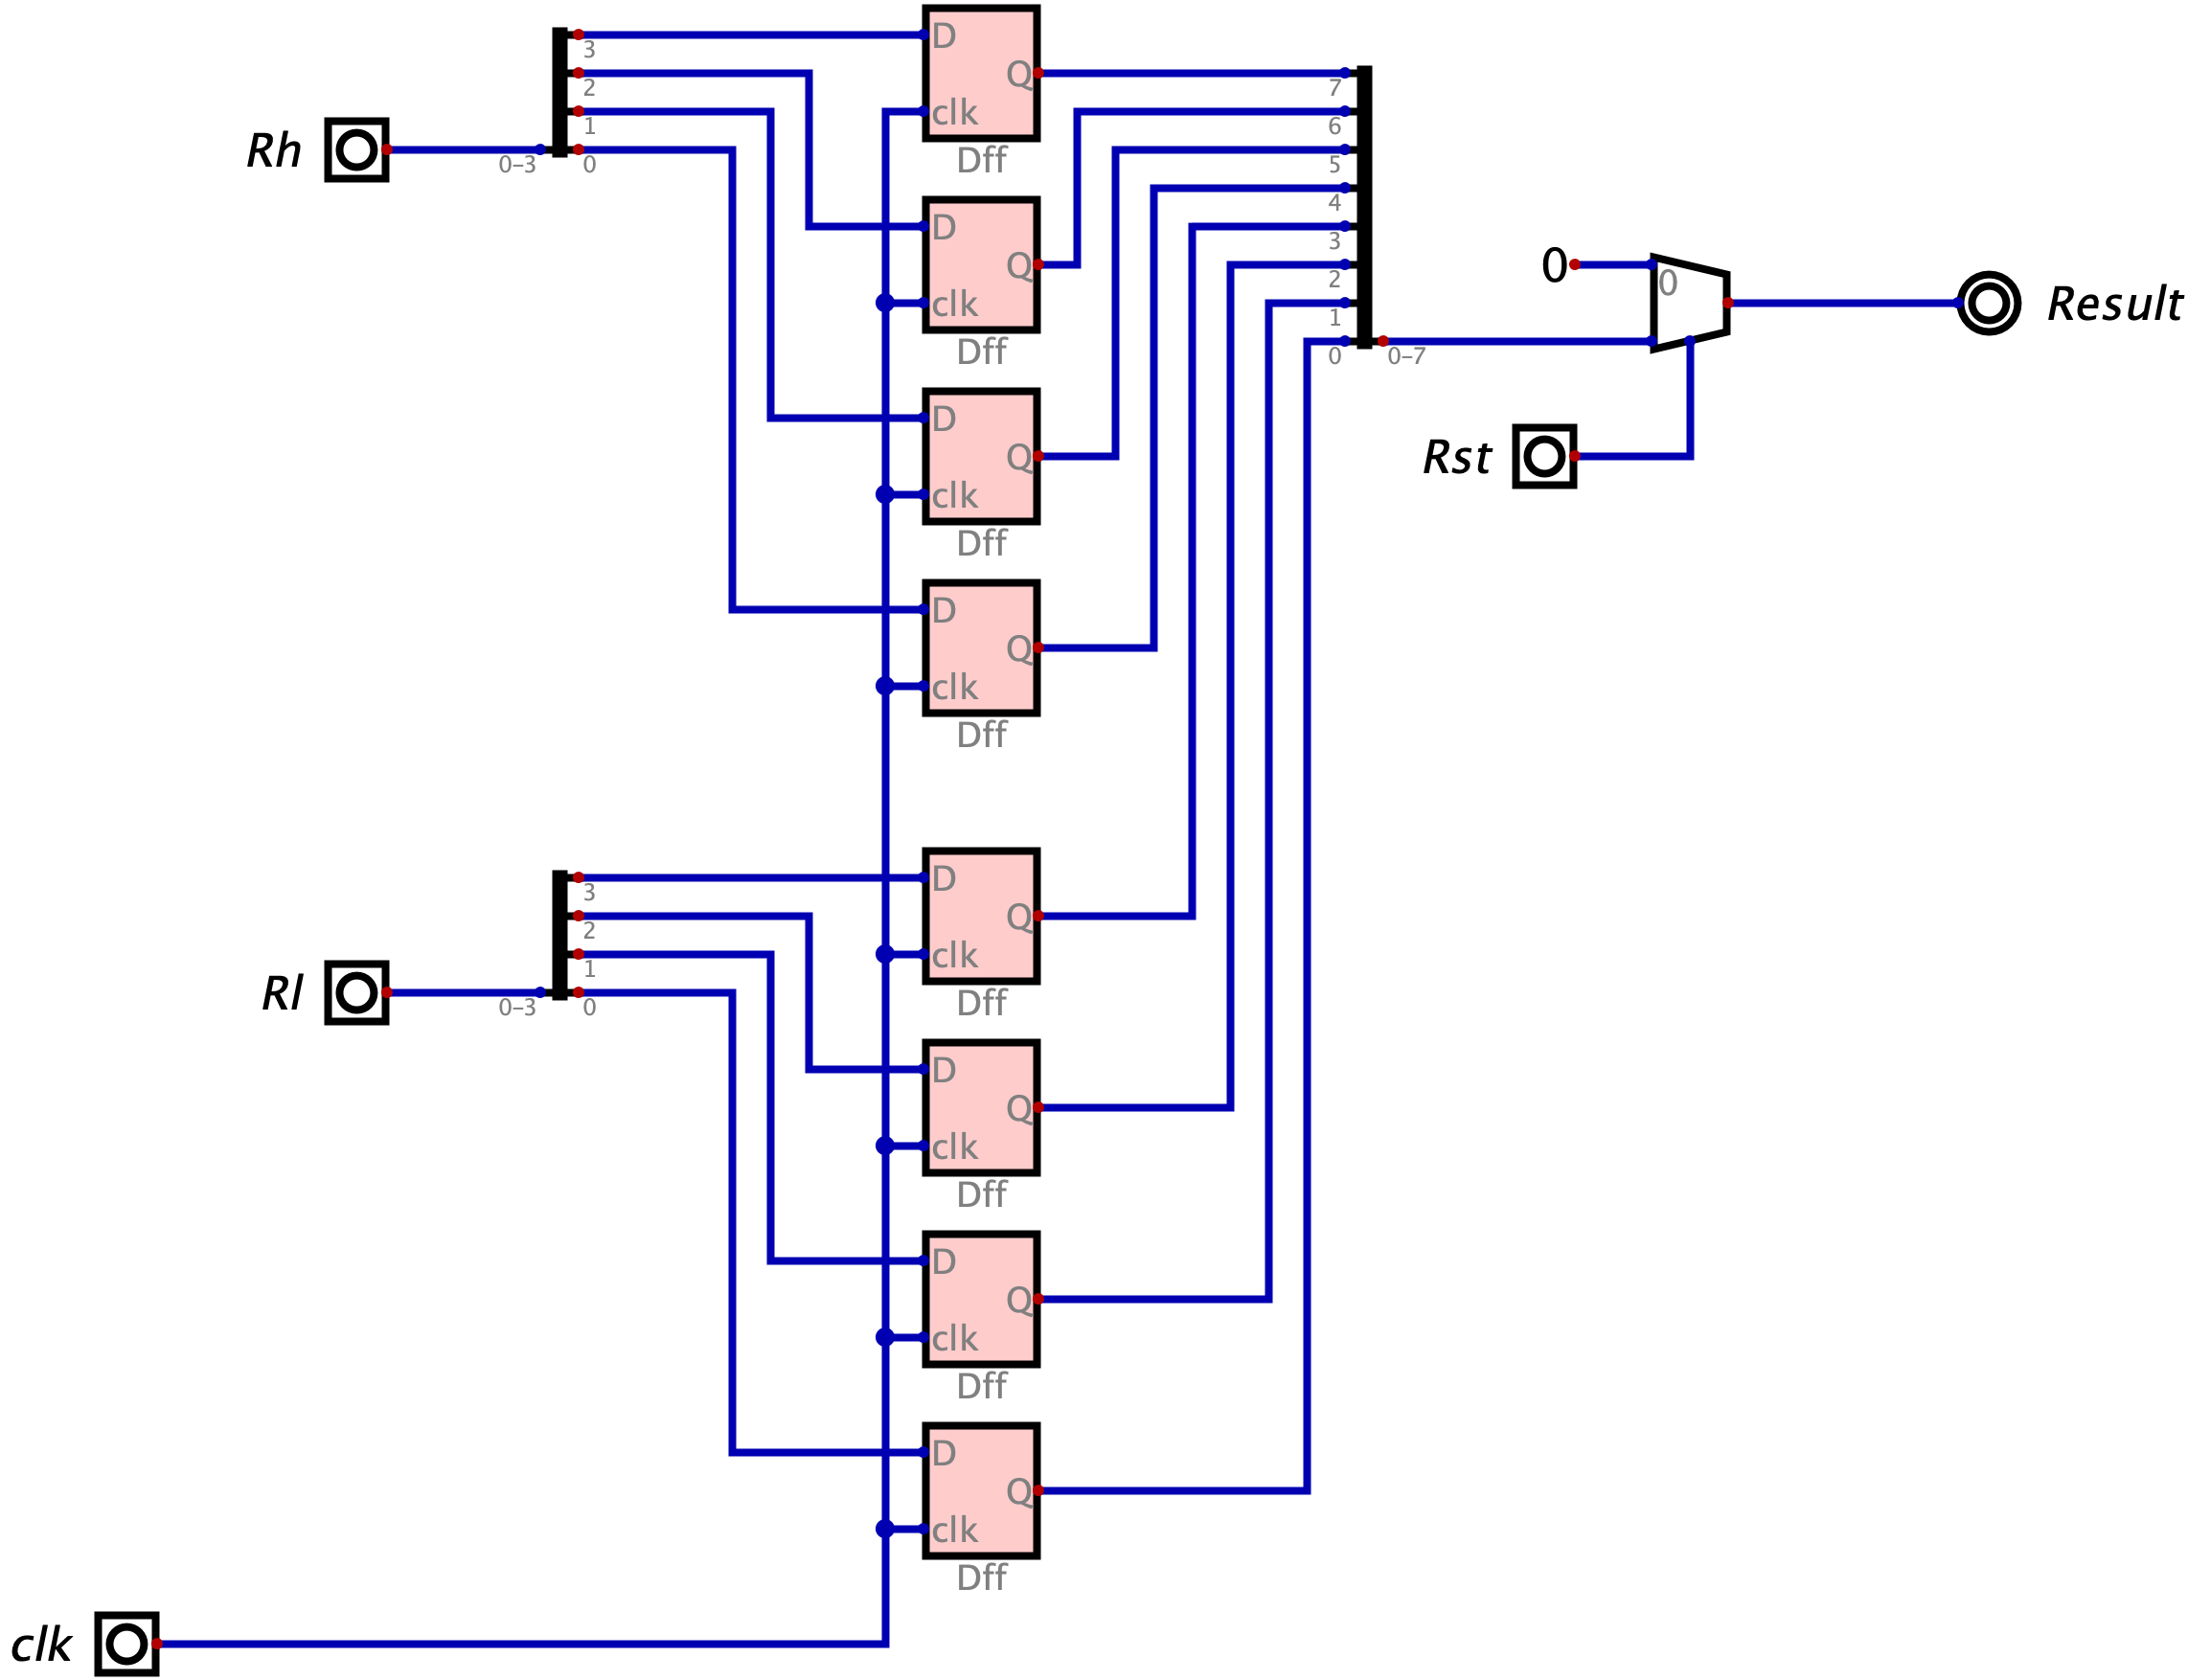
\includegraphics[width=\textwidth]{buffer8bit.png}
		\caption{Connector (8-bit Buffer) subcircuit}
		\label{fig:buffer8bit}
	\end{minipage}
\end{figure}

\begin{figure}[h!]
	\centering
	\begin{minipage}{0.52\textwidth}
		\centering
		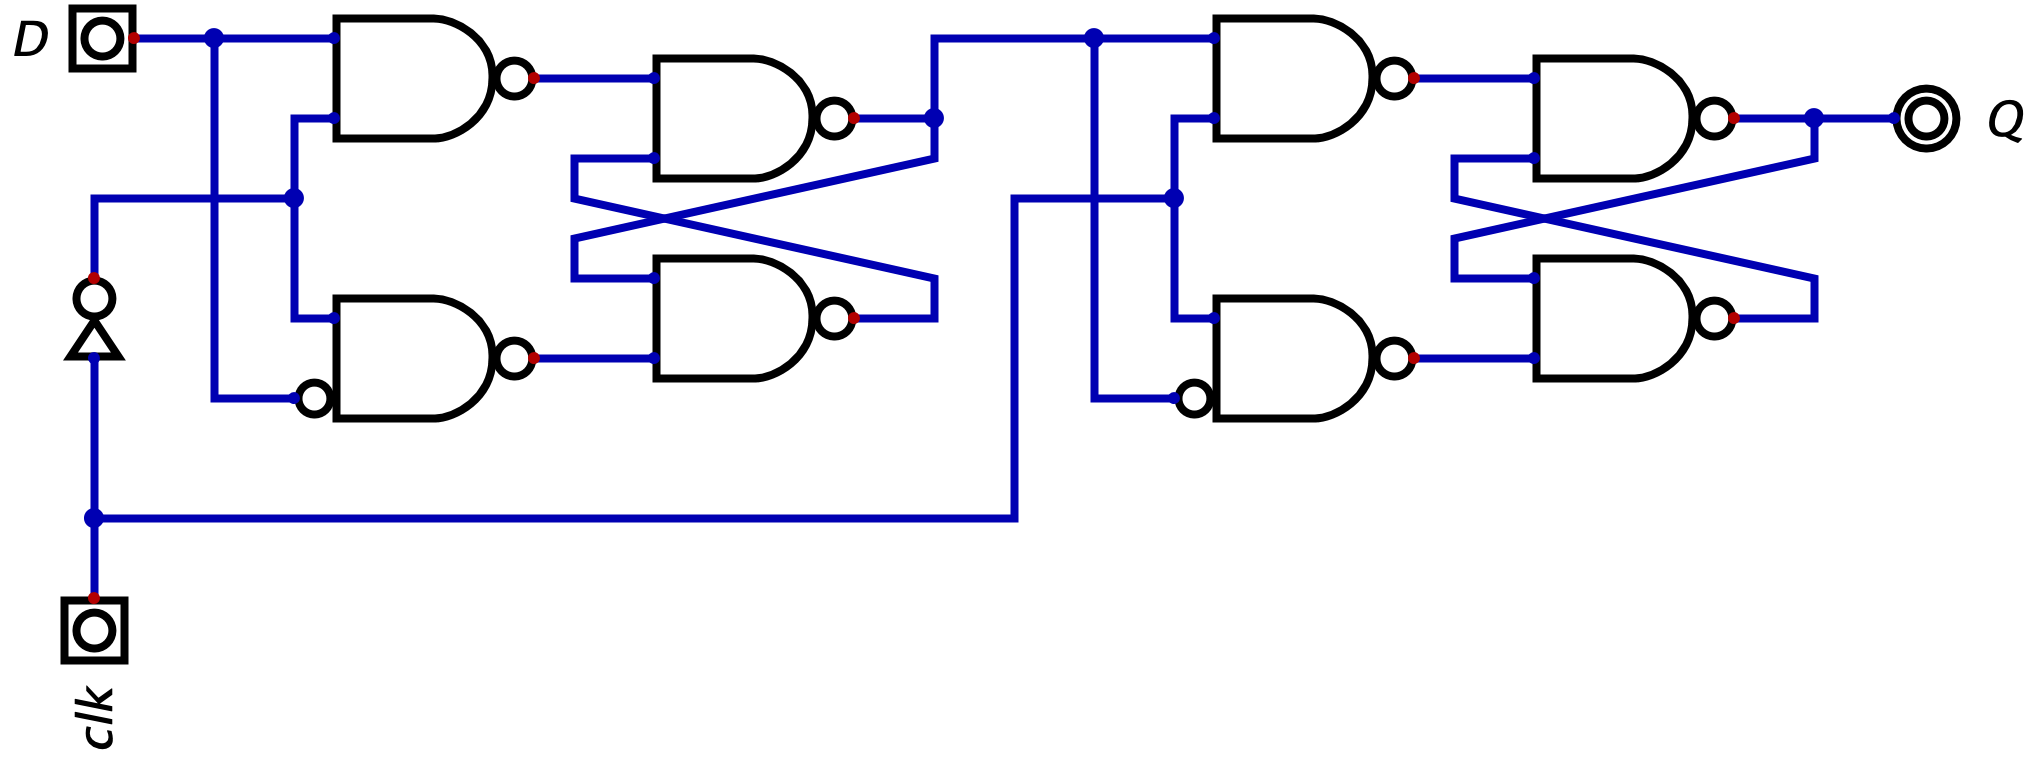
\includegraphics[width=\textwidth]{Dff.png}
		\caption{Master-slave D Flip-Flop subcircuit}
		\label{fig:Dff}
	\end{minipage}
	\hfill
	\begin{minipage}{0.45\textwidth}
		\centering
		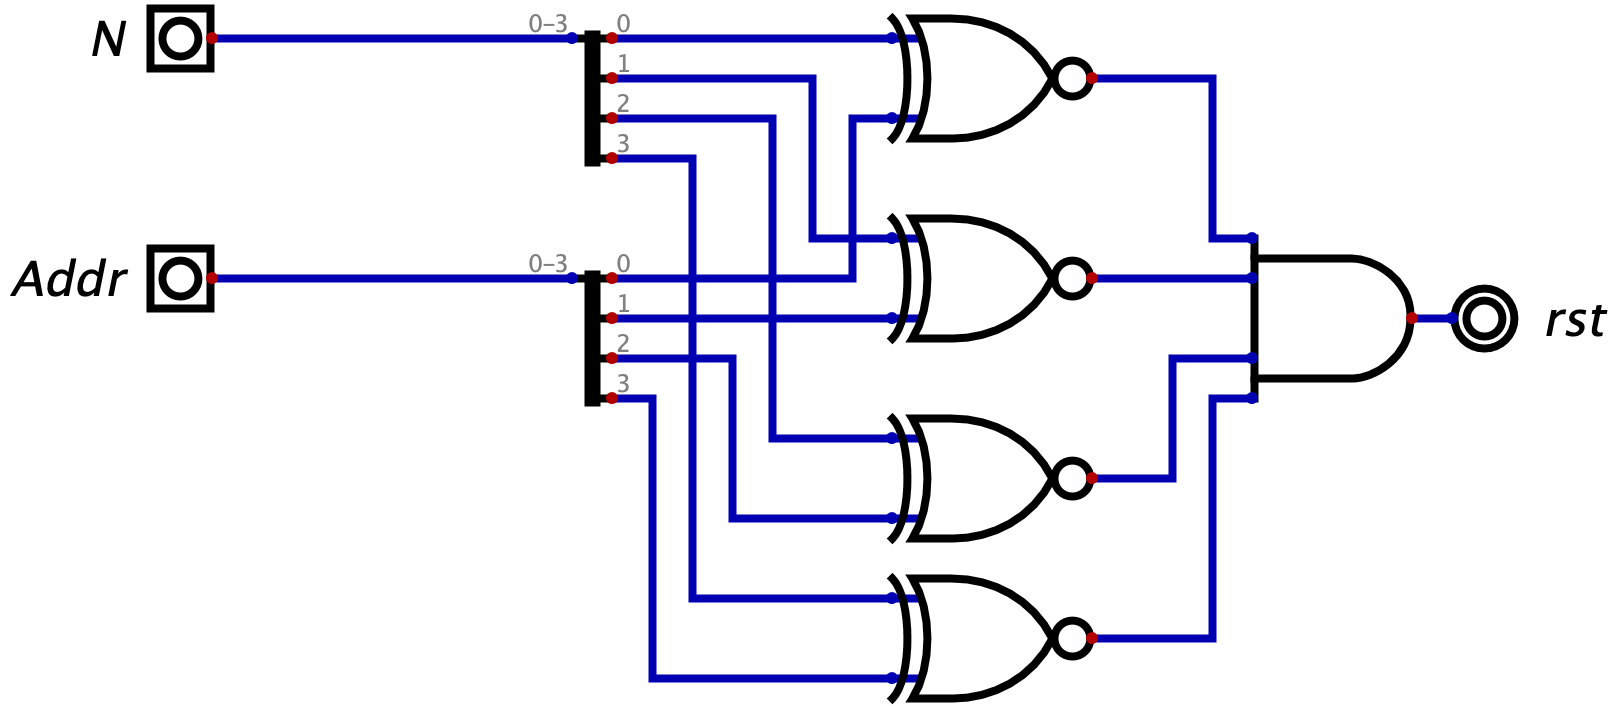
\includegraphics[width=\textwidth]{isMax.png}
		\caption{\texttt{isMax} module (Part of the FSM) subcircuit}
		\label{fig:isMax}
	\end{minipage}
\end{figure}

\begin{figure}[h!]
	\centering
	\includegraphics[width=0.4\textwidth]{EEPROM.png}
	\caption{Data Storage Part (EEPROM) subcircuit}
	\label{fig:EEPROM}
\end{figure}


\clearpage
\section{VHDL Codes}
\label{app:c}

\subsection{VHDL Codes for PART II}
\lstinputlisting[caption={Behavioural description of 2-bit adder}, label={lst:2bit_adder}, language=VHDL, style=customvhdl]{../vhdl/behavior/adder2bit.vhdl} % VHDL code from file

\lstinputlisting[caption={Behavioural description of 4-bit adder}, label={lst:4bit_adder}, language=VHDL, style=customvhdl]{../vhdl/behavior/adder4bit.vhdl} % VHDL code from file

\subsection{VHDL Behavioural Description for Each Block in PART III}
\label{app:c2}

\subsubsection{Counter}

\lstinputlisting[caption={\texttt{DIG\_Counter} as the subcircuit for \texttt{RhCount} and \texttt{main}}, label={lst:DIG_Counter}, language=VHDL, style=customvhdl]{../vhdl/behavior/DIG_Counter.vhdl} % VHDL code from file

\lstinputlisting[caption={\texttt{RhCount} is just an instantiation of \texttt{DIG\_Counter}}, label={lst:RhCount}, language=VHDL, style=customvhdl]{../vhdl/behavior/RhCount.vhdl} % VHDL code from file

\subsubsection{Decoder}

\lstinputlisting[caption={\texttt{DECODER\_4} as the subcircuit for \texttt{EEPROM} and \texttt{main}}, label={lst:DECODER_4}, language=VHDL, style=customvhdl]{../vhdl/behavior/DECODER_4.vhdl} % VHDL code from file

\subsubsection{Multiplexer}

\lstinputlisting[caption={\texttt{MUX\_GATE\_BUS\_1} as the subcircuit for \texttt{EEPROM}, \texttt{buffer8bit}, \texttt{buffer4bit} and \texttt{main}}, label={lst:MUX_GATE_BUS_1}, language=VHDL, style=customvhdl]{../vhdl/behavior/MUX_GATE_BUS_1.vhdl} % VHDL code from file

\subsubsection{D Flip-Flop}

\lstinputlisting[caption={\texttt{Dff} as the subcircuit for \texttt{EEPROM}, \texttt{buffer8bit}, \texttt{buffer4bit} and \texttt{main}}, label={lst:Dff}, language=VHDL, style=customvhdl]{../vhdl/behavior/Dff.vhdl} % VHDL code from file

\subsubsection{EEPROM (Data Storage Part)}

\lstinputlisting[caption={\texttt{EEPROM} as the subcircuit for \texttt{main}}, label={lst:EEPROM}, language=VHDL, style=customvhdl]{../vhdl/behavior/EEPROM.vhdl} % VHDL code from file

\subsubsection{FSM (Control Unit)}

\lstinputlisting[caption={\texttt{isMax} as the subcircuit for \texttt{main}, providing control signals}, label={lst:isMax}, language=VHDL, style=customvhdl]{../vhdl/behavior/isMax.vhdl} % VHDL code from file

\subsubsection{Counter (Higher 4 bits adder)}

\lstinputlisting[caption={\texttt{buffer4bit} as the subcircuit for \texttt{main}}, label={lst:buffer4bit}, language=VHDL, style=customvhdl]{../vhdl/behavior/buffer4bit.vhdl} % VHDL code from file

\subsubsection{Connector (8-bit Buffer)}

\lstinputlisting[caption={\texttt{buffer8bit} as the subcircuit for \texttt{main}}, label={lst:buffer8bit}, language=VHDL, style=customvhdl]{../vhdl/behavior/buffer8bit.vhdl} % VHDL code from file

\subsection{VHDL Codes for the Complete Generalised Adder}
\label{app:c3}

\lstinputlisting[caption={Structural description of the complete generalised adder reusing the codes in Appendix~\ref{app:c2}}, label={lst:main}, language=VHDL, style=customvhdl]{../vhdl/structural/main.vhdl} % VHDL code from file

\end{appendix}


\end{document}